\subsection{Протокол MTI/A(0)}\label{section-protocols-mti}\index{протокол|MTI/A(0)|(}
\selectlanguage{russian}

В 1986 году Ц.~Мацумото (\langen{Tsutomu Matsumoto}), И.~Такашима (\langen{Youichi Takashima}) и Х.~Имаи (\langen{Hideki Imai}) предложили несколько алгоритмов, позже названных семейством протоколов MTI (\cite{Matsumoto:Tsutomu:Imai:1986}). За счёт предварительного распространения открытых ключей обоих сторон они обеспечивали неявную аутентификацию ключа (цель G7). То есть сессионный ключ гарантированно мог получить только владельцы соответствующих открытых ключей. Мы рассмотрим одного из представителей данного семейства -- протокол MTI/A(0) (рис.~\ref{fig:key_distribution-mti}).

Предварительно стороны договорились об общих параметрах системы $p$ и $g$, где $p$ -- большое простое число, а $g$ -- примитивный элемент поля $\Z_p^*$.

Каждая из сторон (Алиса и Боб) сгенерировала пару из закрытого и открытого ключей:
\[\begin{array}{ll}
    Alice: & ~ a, ~~ K_A = g^a \bmod p, \\
    Bob: & ~ b, ~~ K_B = g^b \bmod p. \\
\end{array}\]

\begin{figure}
    \centering
    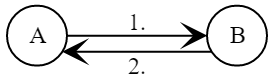
\includegraphics[width=0.5\textwidth]{pic/key_distribution-mti}
    \caption{Взаимодействие участников в протоколе MTI/A(0)\label{fig:key_distribution-mti}}
\end{figure}

\begin{protocol}
    \item[(1)] Алиса сгенерировала случайное число $R_A: ~ 2\leq R_A\leq p-1$
    \item[{}] $ Alice \to \left\{ g^{R_A} \bmod p \right\} \to Bob$
    \item[(2)] Боб сгенерировал случайное число $R_B: ~ 2\leq R_B\leq p-1$
    \item[{}] Боб вычислил сеансовый ключ $K = (g^{R_A})^b \cdot K_A^{R_B} \bmod p$
    \item[{}] $ Bob \to \left\{ g^{R_B} \bmod p \right\} \to Alice$
    \item[(3)] Алиса вычислила сеансовый ключ $K = (g^{R_B})^a \cdot K_B^{R_A} \bmod p$
\end{protocol}

Если открытые ключи $K_A$ и $K_B$ соответствуют своим закрытым ключам $a$ и $b$, то вычисленные участниками сессионные ключи совпадают:
\[\begin{array}{lll}
    (g^{R_A})^b \cdot K_A^{R_B} \bmod p & = & g^{b R_A + a R_B} \bmod p, \\
    (g^{R_B})^a \cdot K_B^{R_A} \bmod p & = & g^{a R_B + b R_A} \bmod p.
\end{array}\]

Из-за сложности задачи дискретного логарифмирования злоумышленник не сможет получить $a, R_A$ или $b, R_B$ из передаваемых сообщений, а предварительная публикация открытых ключей гарантирует, что сессионный ключ получат только легальные пользователи. Случайный выбор $R_A$ и $R_B$ гарантирует, что обе стороны могут быть уверены в создании нового сессионного ключа в каждом сеансе протокола.

Как и другие представители криптосистем-протоколов, MTI не разрабатывался с учётом возможности компрометации закрытых <<мастер>>-ключей $a$ и $b$ (цель G9).

\index{протокол|MTI/A(0)|)}